\subsection{Secciones de la página web}

    En esta subsección se dará una breve explicación de cada sección de la plataforma web y se acompañará de una imagen.

    \begin{itemize}
        \item Home

        Es la página web que visualiza un usuario no logueado en el sistema donde puede registrarse en ella, recordar la contraseña en caso de que la haya olvidado o registrarse.

        Además, también se muestra información pública sobre los objetivos, la misión y la visión del proyecto.

            \begin{figure}[H]
                \centering
                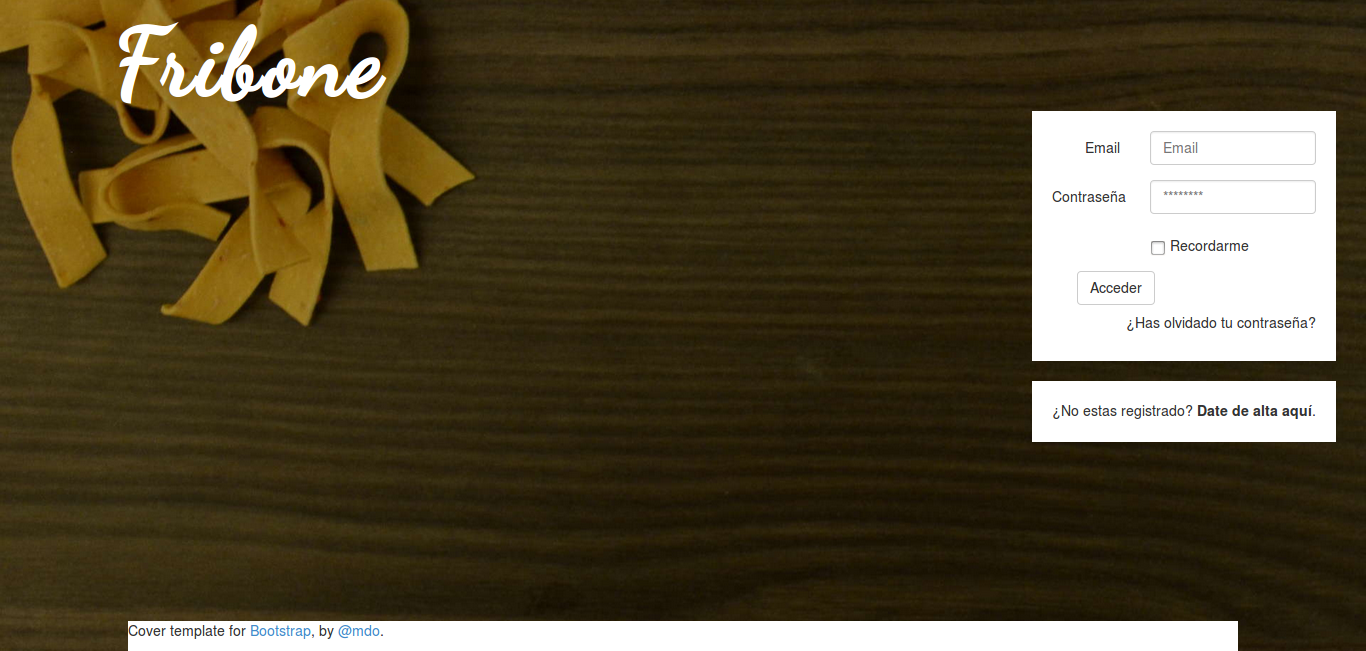
\includegraphics[keepaspectratio,width=0.9\textwidth]{fribone-web-home.png}
                \caption{Web - Home pública}\label{fig:fribone-web-home}
            \end{figure}

        \item Zona privada de usuario

            Esta zona solo es accesible cuando un usuario registrado en la plataforma web se encuentra logueado en el sistema. En caso de no estarlo, se redirije a la Home pública.

            La zona privada se encuentra formada de las siguientes secciones:

            \begin{itemize}
                \item Frigorífico

                Es una de las secciones más importantes de toda la web ya que permite visualizar rapidamente los productos que se tienen en el frigorífico.

                \begin{figure}[H]
                    \centering
                    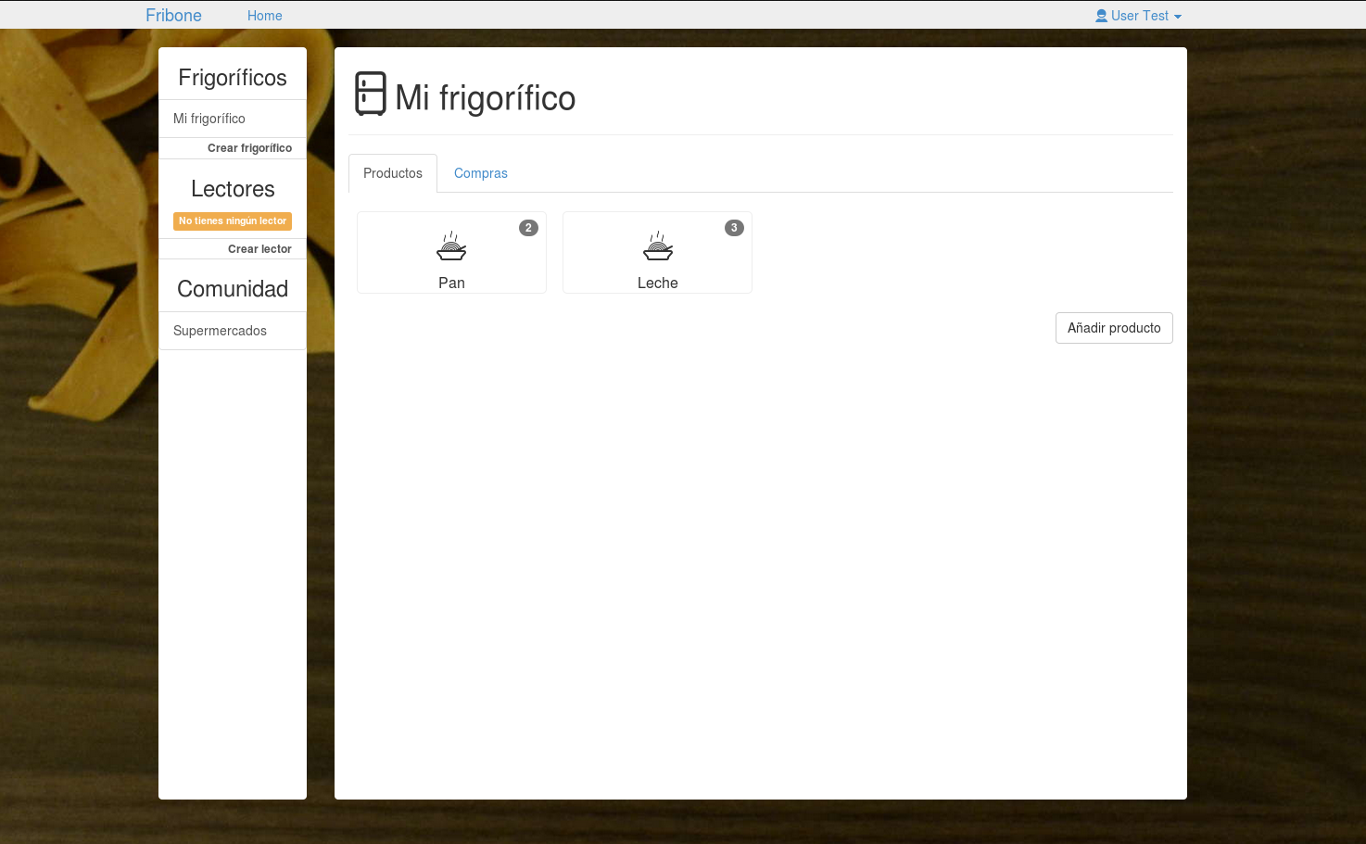
\includegraphics[keepaspectratio,width=0.9\textwidth]{fribone-web-frigorifico.png}
                    \caption{Web - Sección frigorífico}\label{fig:fribone-web-frigorifico}
                \end{figure}

                \parpic[r][]{
                    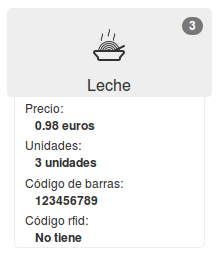
\includegraphics[keepaspectratio,width=0.15\textwidth]{fribone-web-detalles-producto-frigorifico.png}
                    \label{fig:fribone-web-detalles-producto-frigorifico}
                }

                Se puede clickar en cada uno de los productos que se dispongan en el frigorífico para consultar más información acerca de cada uno de los productos (Precio, unidades, código de barras y código rfid).

                \item Compras realizadas

                Las compras se crean automáticamente al añadir productos al frigorífico, sea desde la web o desde el componente hardware realizado con arduino.

                Al introducir un producto se busca si hay una compra creada en la última media hora, si es así, el producto se mete a dicha compra, si no se crea una nueva compra. En resumen, una compra engloba todos los productos introducidos en un rango de tiempo de media hora.

                \begin{figure}[H]
                    \centering
                    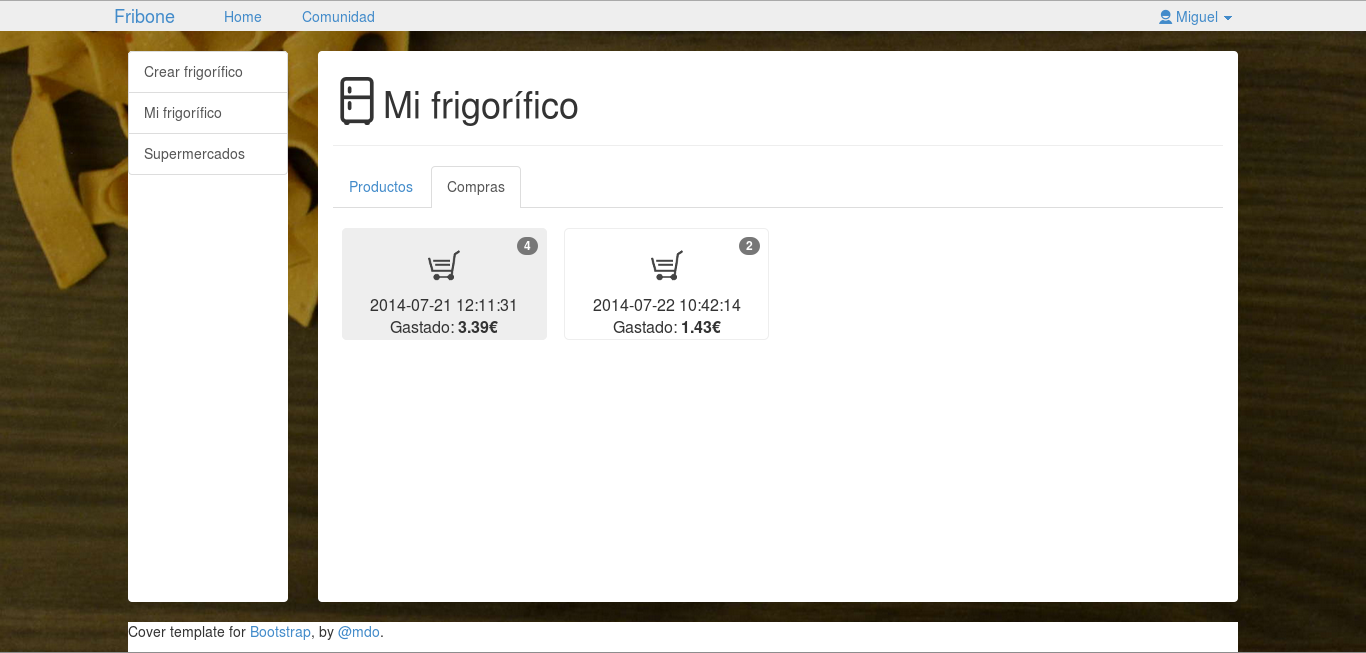
\includegraphics[keepaspectratio,width=0.9\textwidth]{fribone-web-compras.png}
                    \caption{Web - Sección compras}\label{fig:fribone-web-compras}
                \end{figure}

                \item Detalles de una compra

                Además de poder visualizar las compras realizadas, al clickar sobre una de ellas, se nos despliega toda la información de dicha compra; productos introducidos en el frigorífico y el total de la compra.

                \begin{figure}[H]
                    \centering
                    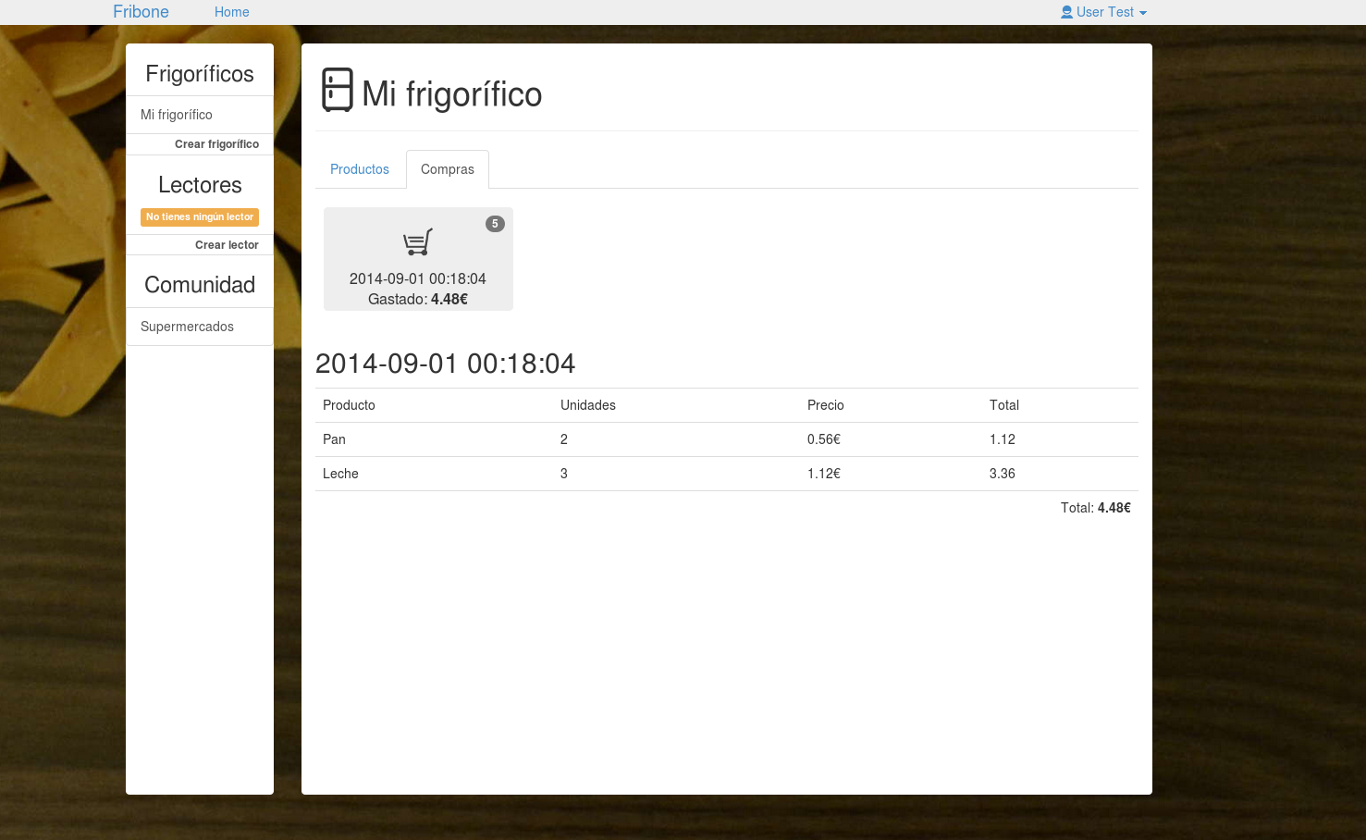
\includegraphics[keepaspectratio,width=0.9\textwidth]{fribone-web-compra.png}
                    \caption{Web - Sección compra}\label{fig:fribone-web-compra}
                \end{figure}

                \item Supermercados

                    La sección de supermercados es común a todos los usuarios, es una zona colaborativa, donde se crean los supermercados existentes para poder añadirles productos.

                    \begin{figure}[H]
                        \centering
                        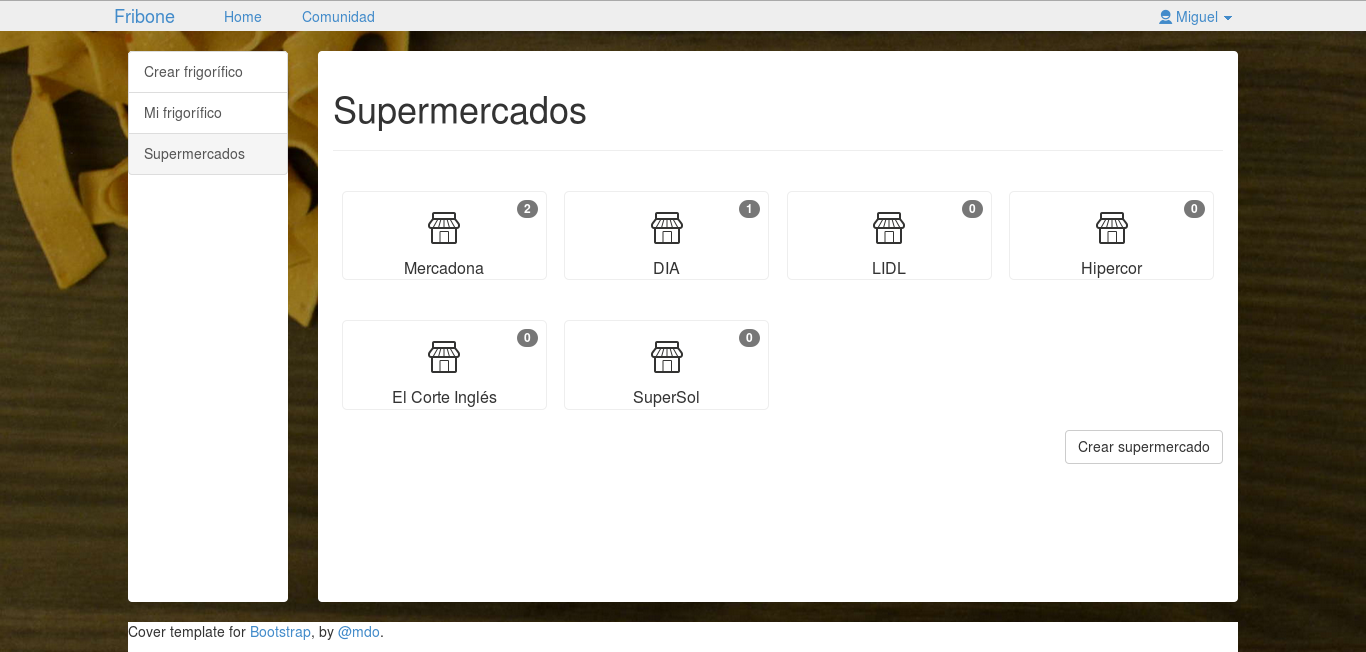
\includegraphics[keepaspectratio,width=0.9\textwidth]{fribone-web-supermercados.png}
                        \caption{Web - Sección supermercados}\label{fig:fribone-web-supermercados}
                    \end{figure}

                \item Vista de un supermercado

                    En esta sección se pueden visualizar los productos que dispone un supermercado, mostrar la información de cada producto y añadirle nuevos productos.

                    \begin{figure}[H]
                        \centering
                        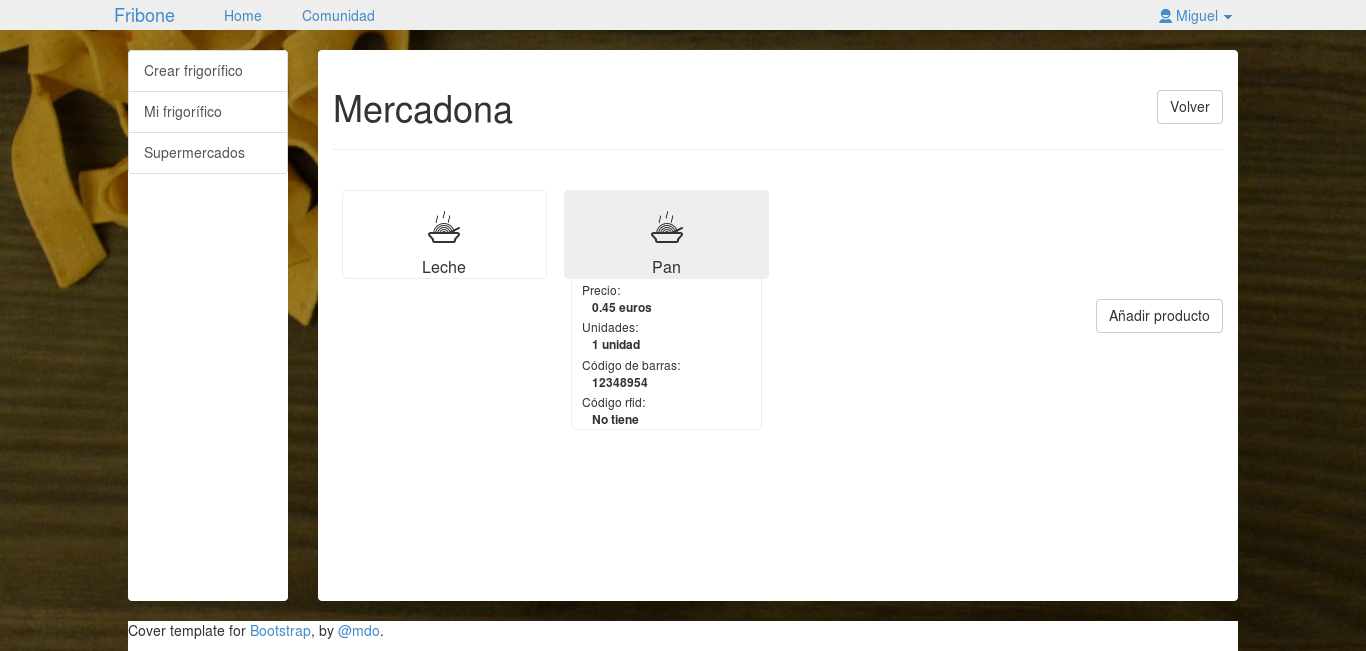
\includegraphics[keepaspectratio,width=0.9\textwidth]{fribone-web-supermercado.png}
                        \caption{Web - Sección de un supermercado}\label{fig:fribone-web-supermercado}
                    \end{figure}

                    Al añadir un producto hay que rellenar el siguiente formulario:

                    \begin{figure}[H]
                        \centering
                        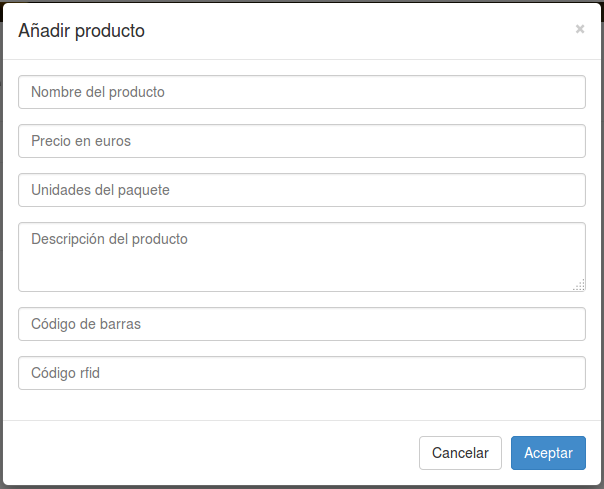
\includegraphics[keepaspectratio,width=0.6\textwidth]{fribone-web-anadir-supermercado.png}
                        \caption{git }\label{fig:fribone-web-anadir-supermercado}
                    \end{figure}

                    Estando disponible para todos los usuarios, así, al agregar dicho producto ya se dispone de toda su información.
            \end{itemize}
    \end{itemize}